\section{Method} \label{sec:method}
%Method
%Prerequisites (things used by all networks)
%Data set (fruit), (landscape)
%Input size (128X128)
%
%Color spaces + which one to use :
%RGB (luminosity not separated from color)
%HSV (circular domain)
%YCbCr (OK)
%CIELab (OK)
%first layer as input, second and third layer as output
%
%Architecture (not what it is but why WE use it)
%General discription (how to colorize an image with an NN)
%Features used by all networks
%ReLu, weight initialization, padding, kernel size
%Feature extraction
%Reconstruct
%Concatenate
%Dilated convolution
%Color generation
%Two feature maps
%blur
%Classification
%k-means
%annealed mean
%gaussian blur
%
%Loss function
%Squared error
%Class rebalancing (histogram dataset)
%Cross entropy
%Class rebalancing
%Architectures used:
%Dahl, Compact, Dahl_classifier, Dahl_zhang, Zhang
%
%Training method
%nesterov momentum
%adadelta

This section contains the various techniques used for the colorization problem.
\subsection{Dataset and Input}

As an input to the network a large amount of images are needed.
However, due to computational limitations, restrictions had to be made.
One of these restrictions resulted in a selection of images based on a certain category; fruit and landscape images.
The fruit dataset contain a rich amount of colors, straining the networks requirements.
This strain is implied by the ambiguity of fruit, being able to contain a vast set of different colors, difficult to predict purely based on a grayscale image.
The landscape dataset is more straight forward, containing less saturated colors and lacks fine details.

The datasets where generated using the popular image website {\color{red} Flickr (XXX)}.
Using their freely available API a program was made that retrieved images in the required resolution and kept track of images retrieved, to avoid duplicates.
The images are then collected in batches and stored in Numpy arrays as input for the network.

The datasets retrieved had to be checked on incorrect images. To solve this problem a web application was made that enabled us to check images on defects. A detailed description can be found in {\color{red}appendix (XXX)}

This resulted in 2 datasets, which are summarized in table \ref{tab:dataset}.

\begin{table}[h!]
	\centering
	\caption{Datasets used for training and validation of the various networks}
	\label{tab:dataset}
	\begin{tabular}{|l|l|l|}
		\hline
		Dataset   & Training Images & Validation images \\ \hline
		Fruit     & 6000            & 1000              \\ \hline
		Landscape & 34000           & 5000              \\ \hline
	\end{tabular}
\end{table}

The network input are 128x128 grayscale images, which can be propagated through the network in different batch sizes. Using batches over the one image at a time reduces computation time, and is a better estimate for the gradient of the loss function of the complete train set \cite{ioffe2015batch}. Making the batch size to large reduces the randomness of the search to the global minimum and results in possible slower convergence.


The input images are converted from an RGB image to a selected colorspace. 
In total three different colorspaces are used; YCbCr, CIELab and HSV. 
The main difference between these colorspaces and RGB is the fact that they inherently have a luminosity layer in their respective colorspace. This luminosity layer is subsequently used as an grayscale input for the network, reducing the needed output of the network to two instead of three for RGB. 
 

YCbCr is a colorspace that contains three layers. Y is the luminosity layer, which is essentially the grayscale input for the network.
The Cb and Cr layers are the chroma blue and chroma red layers respectively.
The reason that this colorspace is used is due to the fact that the luminance layer is a component in the reconstruction of color, reducing the output of the network to two.
The output has to be recombined with the input to retrieve the colorized image.
A visualization of the colorspace can be found in figure (XXX).


Another colorspace that is used is CIELab.
This colorspace shares similarities with the YCbCr color space.
CIELab has three components, L, a and b. The L layer is the luminosity layer, which is used as the grayscale image input.
The a and b layers are the color components. CIELab distinguishes itself from YCbCr due to the fact that this colorspace can, in theory, display all possible electromagnetic frequencies. 
However, the human eye is limited to RGB space. The RGB space plotted in Lab space can be seen in {\color{red} figure XXX}. 


HSV is circular colorspace, where the the components of this colorspace are Hue, Saturation and Value. Value reflects the grayscale component, used as input. The Hue represent the color selected, while the Saturation component determines the color intensity. 
However, most neural network loss function use some form of euclidean distance. This is problematic with the HSV colorspace, due to its circular properties. 

\begin{figure}
	\centering
	\begin{subfigure}[b]{0.32\textwidth}
		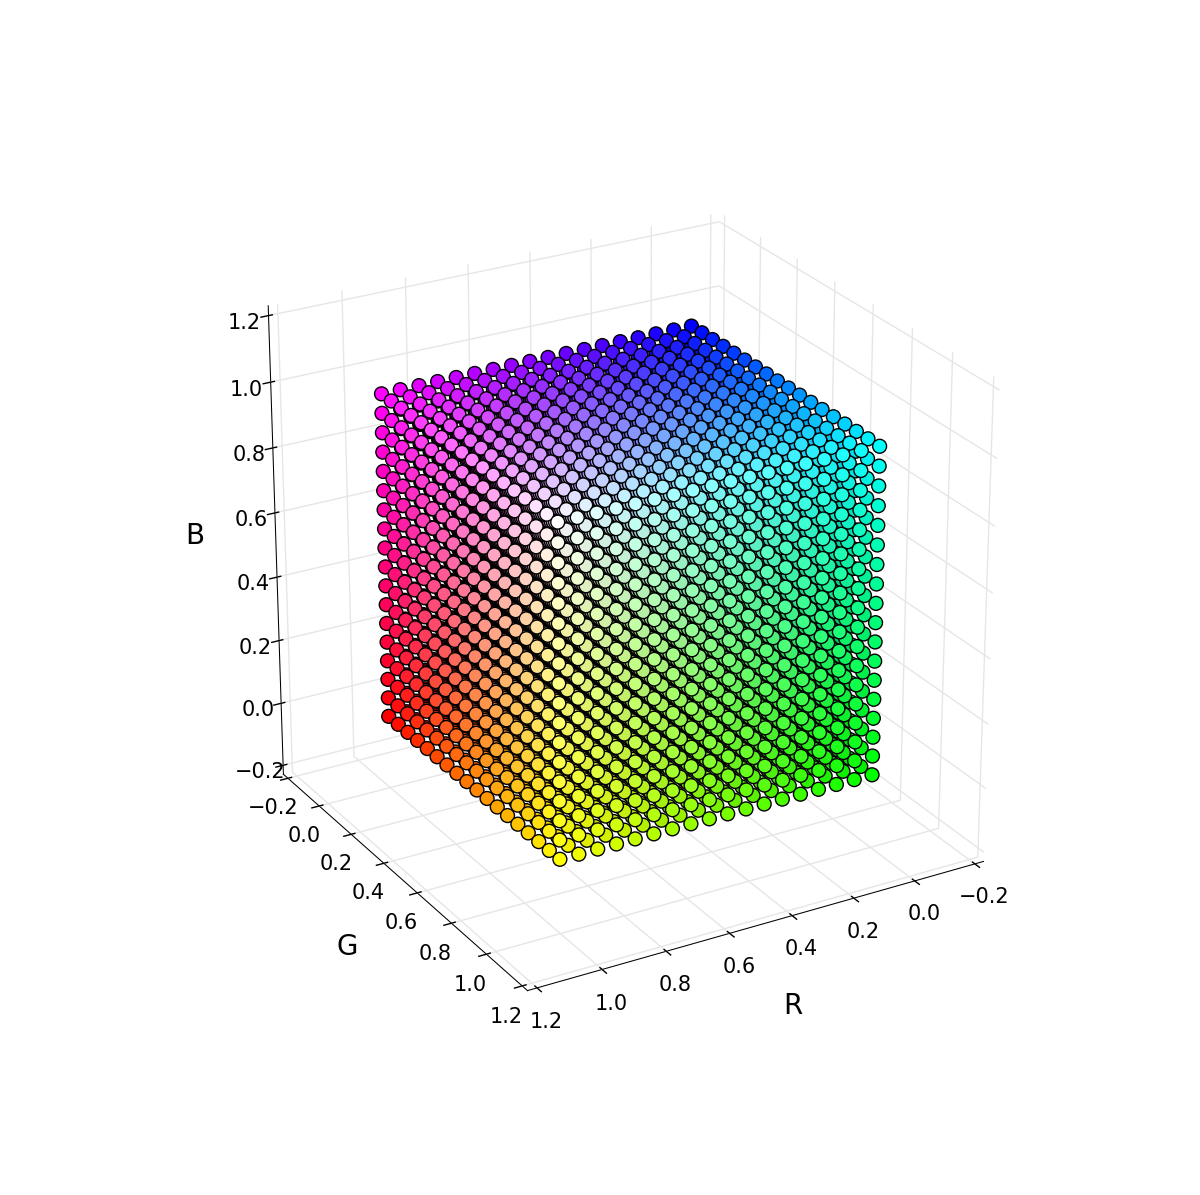
\includegraphics[width=\textwidth,trim={125px 75px 125px 75px},clip]{RGB}
		\caption{The RGB colorspace}
		\label{fig:RGB}
	\end{subfigure}
	~ %add desired spacing between images, e. g. ~, \quad, \qquad, \hfill etc. 
	%(or a blank line to force the subfigure onto a new line)
	\begin{subfigure}[b]{0.32\textwidth}
		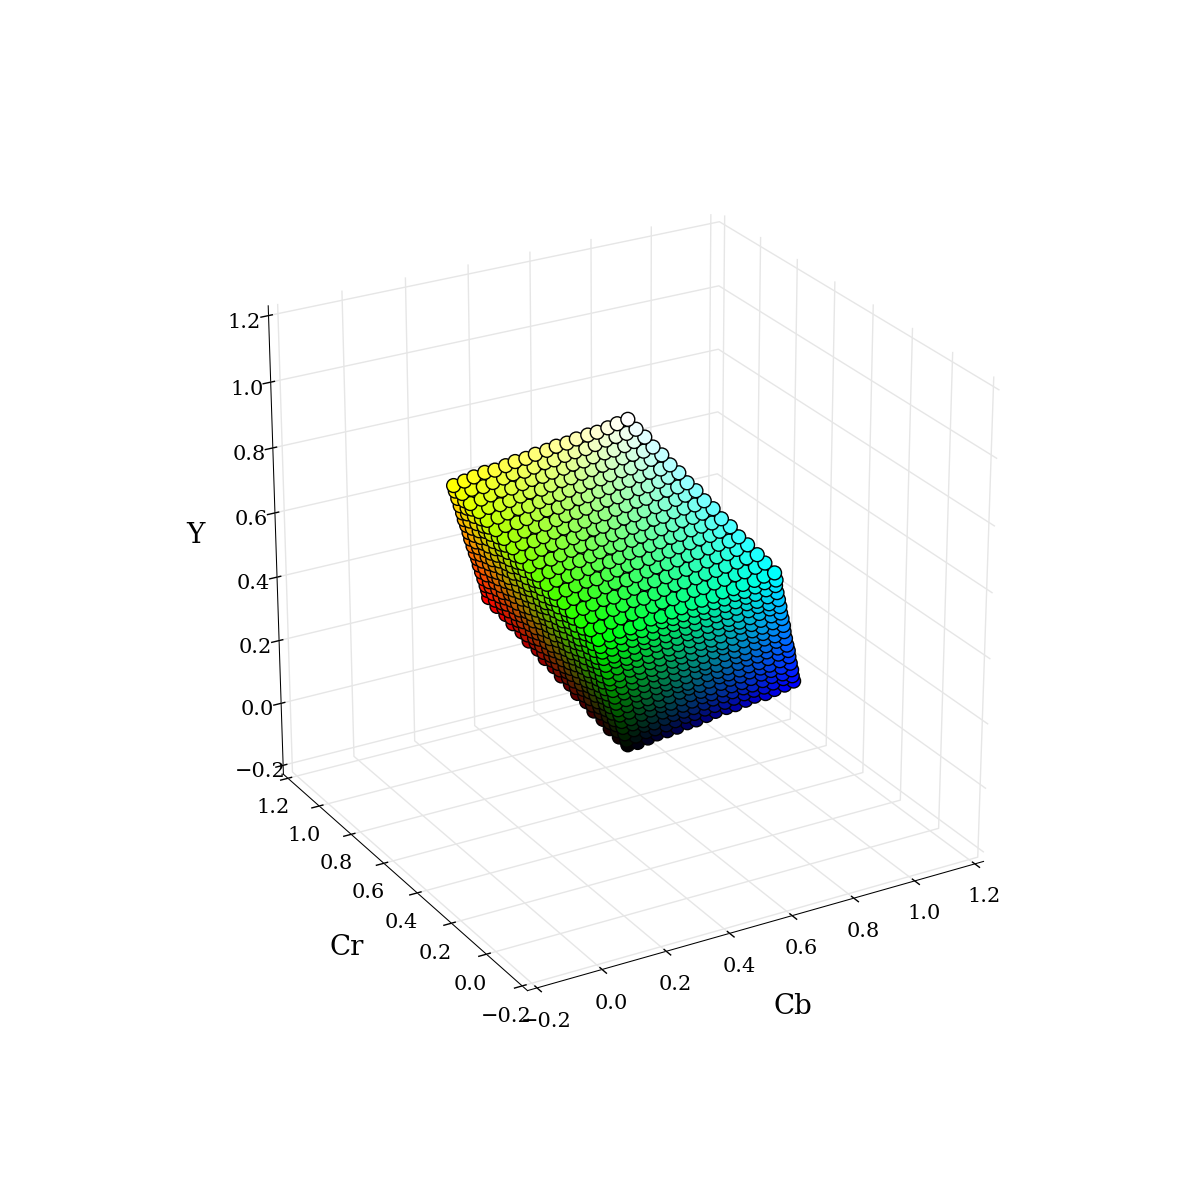
\includegraphics[width=\textwidth,trim={125px 75px 125px 75px},clip]{YCbCr}
		\caption{The RGB colorspace represented in the YCbCr colorspace}
		\label{fig:YCbCr}
	\end{subfigure}
	~ %add desired spacing between images, e. g. ~, \quad, \qquad, \hfill etc. 
	%(or a blank line to force the subfigure onto a new line)
	\begin{subfigure}[b]{0.32\textwidth}
		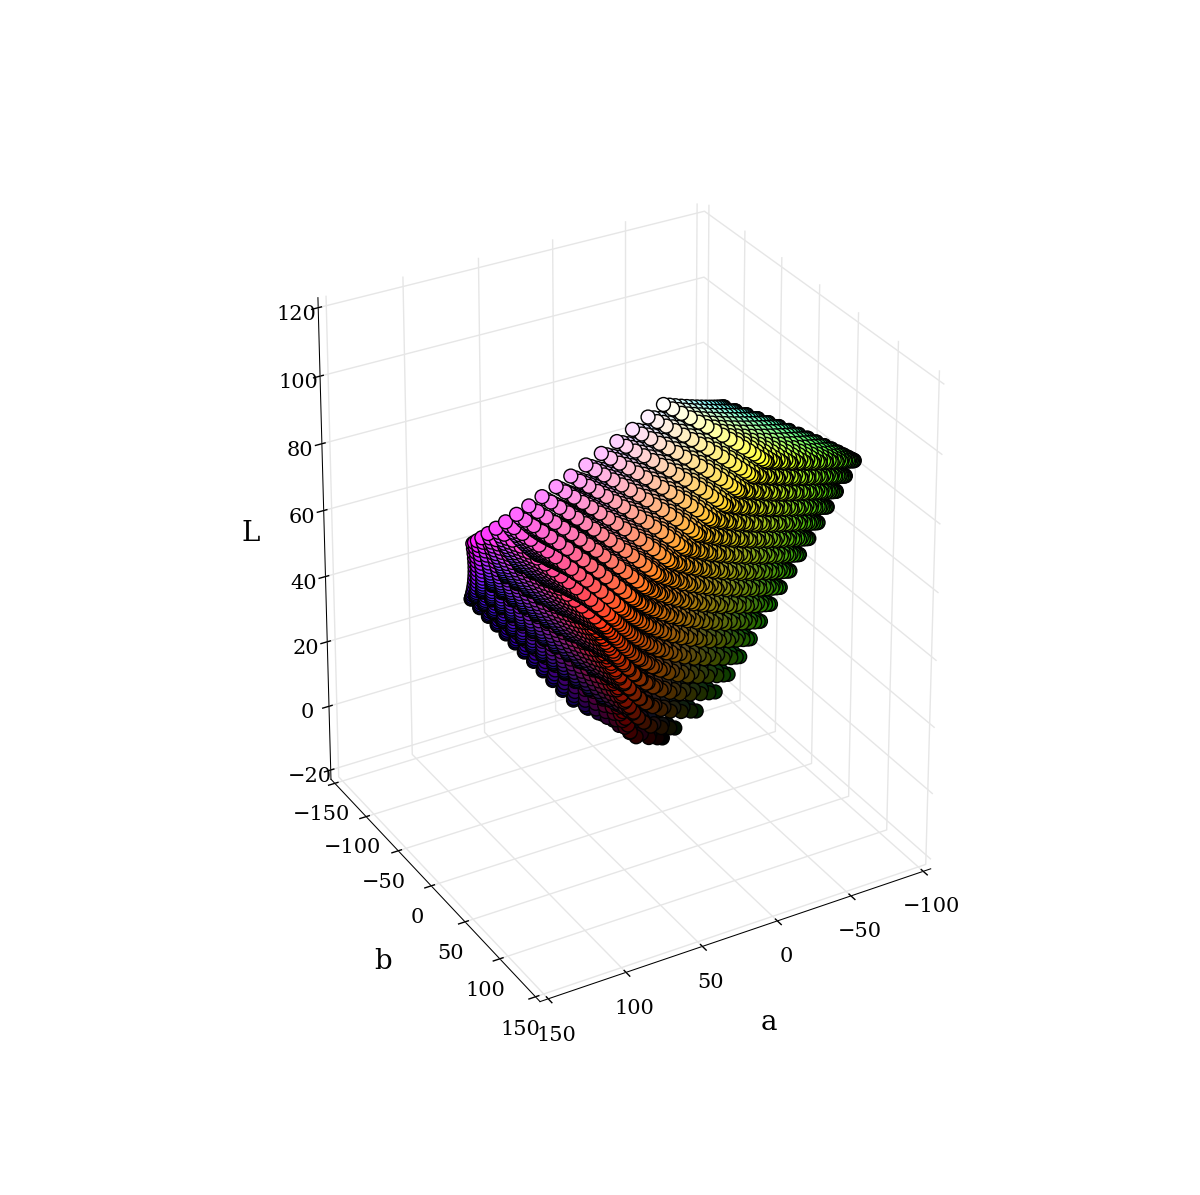
\includegraphics[width=\textwidth,trim={175px 75px 150px 75px},clip]{CIELab}
		\caption{The RGB colorspace represented in the CIELab colorspace}
		\label{fig:CIELab}
	\end{subfigure}
	\caption{The different colorspaces used in the different networks}\label{fig:animals}
\end{figure}


\subsubsection{Neural network properties}
\label{sec:nnproperties}
Neural networks contain a vast amount of different available parameters to tweak the networks behaviour. Throughout the report some of these parameters are kept constant for each network architecture. 

When using a network without pre-trained weights, the networks weights are initialized. This is done using a Glorot Uniform distribution \cite{Glorot} as initialization of the weights. This weight initialization method samples from a uniform distribution with its variance scaled depending on the ingoing and outgoing data. %?

The network consists mainly of convolutional layers. All convolutional layers, except some output layers, use ReLu non-linearities. 

Kernel sizes in the convolutional layers of the network are 3x3 kernels. This kernel size is based upon VGG16's \cite{Simonyan} kernel size.

Stride in the convolutional layers is 1 by default. However, in the classification network {\color{red} ref(XXX)} stride is used as a way to downsample the resolution of the image, comparable to the function of max pooling. %?

Padding is required when using convolutional layers due to the fact that border information of the image is lost when convolving. This property is set to keep the output resolution the same as the input resolution. 


\subsection{Feature Extraction}
To be able to recognize certain objects in grayscale images, object dependent features are extracted. 
This is done in the first part of the convolutional neural network, up until the bottleneck of the network.
To extract these features convolutional layers are used with a varying amount of feature maps. A part of this feature extraction is reducing local features to global features, making them spatially invariant. To accomplish this, Max-pooling is widely used. Another technique available is using an appropriate amount of stride when convolving. {\color{red}reference??}.

This results in spatially invariant feature maps in the bottleneck, only indicating what is in the image, but has no spatial information. To retrieve this spatial information, proper reconstruction of the image has to be done. This is expanded upon in section \ref{sec:reconstruction}.

\subsection{reconstruction}
Before the bottleneck, the image is reduced to a set of features, containing no spatial information. To be able to colorize the image, spatial locations of the object are mandatory. For reconstruction, various methods are used to retrieve the original image resolution.

First of all, the feature maps can be upscaled using linear upscaling. However, to retrieve the original image not only the features but also the information of where those features are coming from have to be retrieved. This is done by concatenating the layers of the same resolution before the bottleneck with the upscaled features after the bottleneck. Then an convolutional layer is used to merge these features in feature maps of the upscaled resolution. This process is repeated until the original image resolution is retrieved.

{\color{red}Another technique used is the use of dilated convolutions.} %Jopie.}

\subsection{Color Generation}
In the final layers of the network, the original image color layers have to be reconstructed. Two different methods are used throughout the paper; Construction using two feature maps and classification.

The construction using two feature maps is a direct result of retrieving the original image resolution through the reconstruction of the image. As a final layer, a convolutional layer is used that maps to two feature maps, which represent the two color layers that are finally used to create a colorized image.

To 





 
\subsection{Model Architectures}
A major part in creating a successful neural network is finding a suitable network architecture. For image classification convolutional neural networks are widely used with success \cite{Krizhevsky,Szegedy,Simonyan}. For our purpose a main feature of the convolutional network is that the image has to be reconstructed again, to retrieve spatial information.

{\color{red} 
In total a set of three convolutional network architectures are used. An architecture based upon Dahl \cite{Dahl}, a pre-trained VGG16 \cite{Simonyan} architecture {\color{red} this is actually Dahl,  not sure about the actual amount of layers used for the reconstruction} and a classification architecture \cite{Zhang}. The architectures of the network are split up in a feature extraction part and a reconstruction part, which will be expanded upon in the following sections.}\\ 
\\%weet neit of je dit mag zeggen..

{\color{red}
\textbf{Feature extraction}

%%Check op diepgang.

\subsubsection{Dahl}%weet geen naam}


This convolutional network is based upon the architecture used by Dahl \cite{Dahl}. It contains several convolutional layers, which use a 3x3 kernel throughout the network. After a set of convolutions a batch normalization is done followed by a max pool layer. Batch normalization is added such that in the reconstruction of the image the concatenated layers are in the same order of magnitude. The architecture was modified to fit the input dimensions. The network is an untrained network, having Glorit uniform distributed \cite{Glorot} initialized weights, meant to be trained simultaneously with the rest of the network. At the bottleneck of the architecture, the resolution of the feature maps are reduced to 16x16 pixels.
 
%Figure toevoegen van het netwerk

\subsubsection{VGG16}
A substantial amount of pre-trained networks are available, trained on the ImageNet classification database. The architecture used is based upon VGG16 \cite{Simonyan}, which uses a 3x3 kernel throughout the network. This network has a proven architecture, and can be obtained with pre-trained weights. Modifications on the network where required to fit the input dimensions. VGG16 is used in classification of RGB images, while our network only needs one input, a grayscale image. The pre-trained weights of the three input maps where averaged to accept a single grayscale input image. The VGG16 architecture features several convolutional layers followed by max pooling. Batch normalization was added before every max pool layer, such that in the later concatenation of the layers the values are in the same order of magnitude. At the bottleneck of the architecture the feature maps have a resolution of 16x16 pixels. 

\subsubsection{Classification}
The classification architecture shares much similarities with the VGG16 architecture. The main difference can be found in the final layers of the network. This is due to the fact that classification is used rather than direct reconstruction of the wanted color layers. This classification is subsequently used to colorize the image. \\
\\
\textbf{Reconstruction}

For reconstruction of the image, linear up-scaling is used. The reconstruction begins after the bottleneck of the convolutional network is reached, where the resolution of the feature maps is 16x16 pixels. The up-scaled information is concatenated with the convolutional layer before the bottleneck that matches the up-scaled layer resolution. Then a convolutional layer is used for feature extraction of the concatenated layer. A batch normalization is applied and the processes is repeated until the original image resolution is retrieved. For both the VGG16 and Dahl based architecture a final output layer is used with a 2 feature map output, which match to the corresponding colour output layers.

For the classification the image is reconstructed to its original resolution. However, first a convolutional layer using a 1x1 kernel is used that has the same amount of feature maps as the required number of possible color classification bins. Then, these feature maps, representing discretized colours, %jopie jou expertise.


A detailed representation with of the various architectures is given in figure {\color{red}(XXX)}}

\subsection{Loss funtion}

\begin{wrapfigure}{r}{0.5\textwidth}
	\vspace{-20pt}
	\begin{center}
		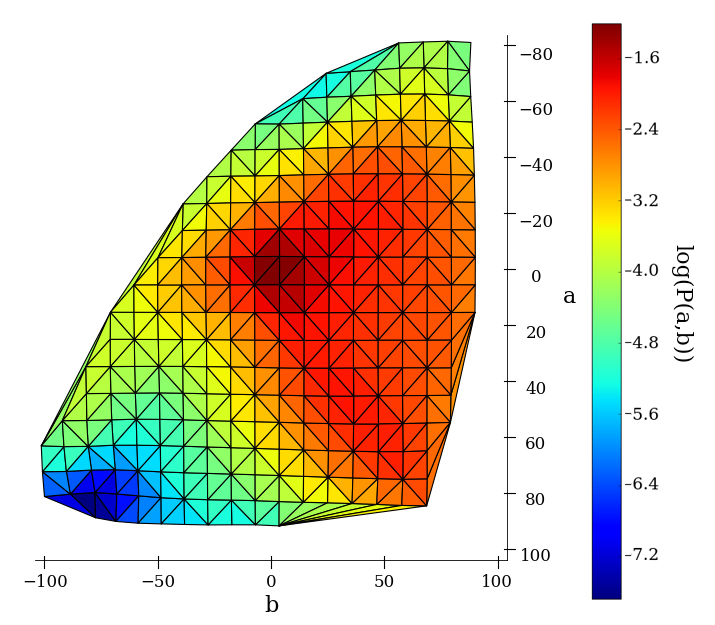
\includegraphics[width=0.48\textwidth]{hist}
	\end{center}
	\caption{\color{red} The histogram of the total fruit dataset}
	\vspace{-10pt}
\end{wrapfigure}

\subsection{Training method}


